\chapter{A Ferramenta de Detecção}
A ferramenta para detecção de botnets foi desenvolvida utilizando o Ambiente de Desenvolvimento Integrado (\textit{Integrated Development Environment} - IDE) \textit{Qt Creator}. A tela inicial do sistema pode ser vista na Figura \ref{fig:initial_screen}.

\begin{figure}
\centering
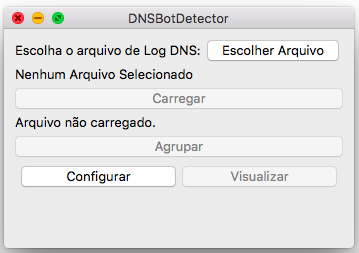
\includegraphics[width=12cm]{initial_screen}
\caption[Tela inicial da Ferramenta]{Tela inicial da Ferramenta} \label{fig:initial_screen}
\end{figure}

Qt é um IDE multi-plataforma que permite desenvolver aplicações com interface gráfica utilizando a linguagem C++ \citep{qtsite}. A escolha de Qt para o desenvolvimento da plataforma foi motivada pelo fato dele ser multi-plataforma, assim como o banco de dados utilizado (PostgreSQL), além do suporte à C++, que foi a linguagem adotada na fase inicial para implementar a preparação de dados.

\section{Documentação de Casos de Uso}
Nesta seção é mostrada a documentação dos casos de usos disponíveis do sistema. O diagrama dos casos de usos pode ser visto na Figura \ref{fig:diagram_use_cases}. A descrição de cada caso de uso é feita ao longo dessa seção. Os passos do Fluxo Básico de Eventos (FBE), são referenciados no Fluxo Alternativo de Eventos.

\begin{table}[]
\centering
\caption{Caso de Uso - Carregar Arquivo de Log DNS}
\label{tb:use_case_load_file}
\begin{tabular}{|lp{10cm}|}
\hline
Nome: & Carregar Arquivo de Log DNS  \\ \hline
Ator: & Usuário   \\ \hline
Pré-condições: & Nenhuma   \\ \hline
\multirow{15}{*}{Fluxo Básico de Eventos:} & 1. O Usuário clica no botão ``Escolher Arquivo''  \\
 & 2. O Sistema exibe uma janela com os arquivos no formato txt presentes no sistema de arquivos do Usuário.  \\
 & 3. O Usuário seleciona um arquivo de log para importar.  \\
 & 4. O Sistema informa o endereço do arquivo selecionado e disponibiliza o botão ``Carregar''. \\
 & 5. O Usuário seleciona a opção ``Carregar'' \\
 & 6. O Sistema exibe um \textit{pop-up} informando que o arquivo está sendo importado para o banco de dados e inicializa a importação dos dados do arquivo para o banco de dados. \\
 & 7. O Sistema retira o \textit{pop-up} informando que o arquivo está sendo importado para o banco de dados e altera o rótulo ``Arquivo não carregado'' para ``Arquivo de Logs Carregado com Sucesso!'' e o caso de uso é encerrado com sucesso.\\ \hline
\multirow{3}{*}{Fluxo Alternativo de Eventos:} & \textbf{(A1) Nenhum Arquivo Selecionado:} No passo 4 do FBE se o Usuário cancelar a seleção de arquivo.\\
 & A1.a) O caso de uso é encerrado com falha.\\ \hline
\multirow{4}{*}{Pós-Condições:} & 1. Os dados contidos no log informado pelo usuário são carregados no banco de dados. \\
 & 2. Os botões ``Agrupar'' e ``Visualizar'' são habilitados.\\
 & 3. O botão ``Carregar'' é desativado.\\
\hline 
\end{tabular}
\end{table}

\begin{figure}
\centering
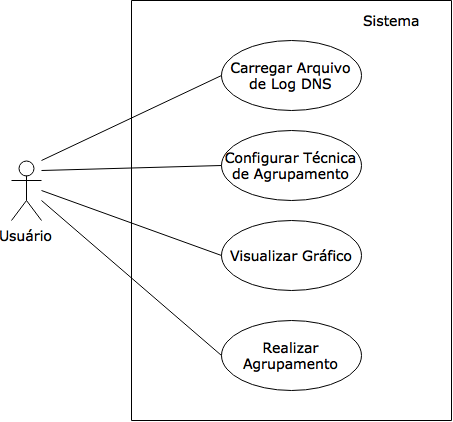
\includegraphics[width=12cm]{diagram_use_cases}
\caption[Diagrama de Casos de Uso]{Diagrama de Casos de Uso} \label{fig:diagram_use_cases}
\end{figure}

\section{Arquitetura do Sistema}
A Figura \ref{fig:program_flow} mostra um diagrama do fluxo básico de funcionamento do sistema.

\begin{figure}
\centering
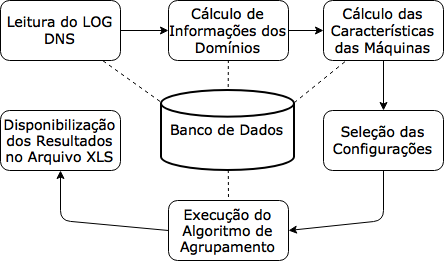
\includegraphics[width=12cm]{program_flow}
\caption[Diagram do Fluxo do Programa]{Diagrama do Fluxo do Programa} \label{fig:program_flow}
\end{figure}
